\documentclass{beamer}
% \usefonttheme{professionalfonts}
\usefonttheme{professionalfonts}
\usepackage{listings}

\usepackage{amsmath}
\usepackage{cancel}
%%%%%%%%%%%%%%%%%%%%%%%%% For making hand-outs %%%%%%%%%%%%%%%%%%%%%%%%%%%
% \documentclass[handout]{beamer}
% \usepackage{pgfpages}
% \pgfpagesuselayout{2 on 1}[a4paper,border shrink=5mm]
%%%%%%%%%%%%%%%%%%%%%%%%%%%%%%%%%%%%%%%%%%%%%%%%%%%%%%%%%%%%%%%%%%%%%%%%%%
\definecolor{inputred}{HTML}{c30e0e}
\definecolor{hiddenblue}{HTML}{2626c9}
\definecolor{outputgreen}{HTML}{008000}
\newcommand{\figheight}{0.72\textheight}
% \usepackage{eulervm}
\usepackage{default}
\usepackage{caption}
\usepackage{booktabs,mathptmx,siunitx}
% \usefonttheme{serif}
\graphicspath{{img/}}
\captionsetup{font=scriptsize, labelfont=scriptsize}


\usepackage{showexpl}

\definecolor{codebg}{HTML}{F3D5F5}

\lstset{language=Python,
breakatwhitespace=false, showspaces=false, showtabs=false, breakatwhitespace=false, breaklines=false, 
backgroundcolor=\color{codebg}}

\lstdefinestyle{highlight}{keywordstyle=\color{blue},
breakatwhitespace=false, showspaces=false, showtabs=false, breakatwhitespace=false, breaklines=false, 
commentstyle=\ttfamily\color{purple}}
\lstdefinestyle{base}{
%   language=Python,
  basicstyle=\ttfamily\color{codebg},
  breakatwhitespace=false, showspaces=false,showstringspaces=false, showtabs=false, breakatwhitespace=false, breaklines=false, 
  keywordstyle=\color{codebg},
  commentstyle=\ttfamily\color{codebg},
  moredelim=**[is][\only<1->{\color{black}\lstset{style=highlight}}]{@}{@},
  moredelim=**[is][\only<1->{\color{black}\lstset{style=highlight}}]{@1}{@},
  moredelim=**[is][\only<2->{\color{black}\lstset{style=highlight}}]{@2}{@},
  moredelim=**[is][\only<3->{\color{black}\lstset{style=highlight}}]{@3}{@},
  moredelim=**[is][\only<4->{\color{black}\lstset{style=highlight}}]{@4}{@},
  moredelim=**[is][\only<5->{\color{black}\lstset{style=highlight}}]{@5}{@},
  moredelim=**[is][\only<6->{\color{black}\lstset{style=highlight}}]{@6}{@},
  moredelim=**[is][\only<7->{\color{black}\lstset{style=highlight}}]{@7}{@},
  moredelim=**[is][\only<8->{\color{black}\lstset{style=highlight}}]{@8}{@},
  moredelim=**[is][\only<9->{\color{black}\lstset{style=highlight}}]{@9}{@}, 
  moredelim=**[is][\only<10->{\color{black}\lstset{style=highlight}}]{@10}{@}, 
  moredelim=**[is][\only<11->{\color{black}\lstset{style=highlight}}]{@11}{@}, 
  moredelim=**[is][\only<12->{\color{black}\lstset{style=highlight}}]{@12}{@}, 
  moredelim=**[is][\only<1>{\color{black}\lstset{style=highlight}}]{~}{~},
  moredelim=**[is][\only<1>{\color{black}\lstset{style=highlight}}]{~1}{~},
  moredelim=**[is][\only<2>{\color{black}\lstset{style=highlight}}]{~2}{~},
  moredelim=**[is][\only<3>{\color{black}\lstset{style=highlight}}]{~3}{~},
  moredelim=**[is][\only<4>{\color{black}\lstset{style=highlight}}]{~4}{~},
  moredelim=**[is][\only<5>{\color{black}\lstset{style=highlight}}]{~5}{~},
  moredelim=**[is][\only<6>{\color{black}\lstset{style=highlight}}]{~6}{~},
  moredelim=**[is][\only<7>{\color{black}\lstset{style=highlight}}]{~7}{~},
  moredelim=**[is][\only<8>{\color{black}\lstset{style=highlight}}]{~8}{~},
  moredelim=**[is][\only<9>{\color{black}\lstset{style=highlight}}]{~9}{~}
%   texcl=true,escapebegin=\hskip-6cm\color{red}
}

\begin{document}



\begin{frame}
% % \frametitle{What is programming?}
% \framesubtitle{It is like use using any other language!}
% 
% ``Getting an education was a bit like a communicable sexual disease. It made you unsuitable for a lot of jobs and then you had the urge to pass it on.''
% \\ \
\centering\Huge Block Practical: Connectionist models and cognitive processes
\vfill \huge
\centering Part 2: \textbf{Introduction to artificial neural networks} \large
\vfill
\textit{
Olivia Guest }

% -- \textit{Terry Pratchett}
\end{frame}


\begin{frame}
\frametitle{What is a neural network?}
\framesubtitle{A mathematical model}
 \begin{columns}[T]
    \begin{column}{.45\textwidth} 
     \ \\ 
     \ \\
\begin{itemize}[<+->]
\item Inspired by the nervous system \\ \
 \item A set of \emph{units}, connected by \emph{weights} \\ \
\item The network \emph{runs} by passing \emph{activations} from the \emph{input} (to the \emph{hidden}) to the \emph{output} units \\ \
\end{itemize}
\end{column}
\begin{column}{.55\textwidth}
\begin{figure}[t]
 \begin{flushleft}

 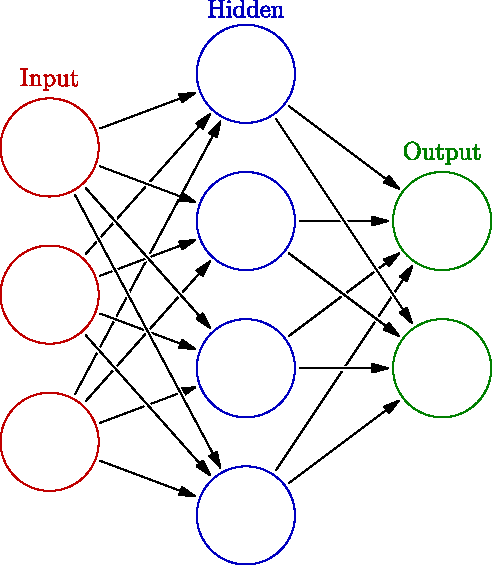
\includegraphics[height = \figheight]{./fig/3-layer.pdf}
 \end{flushleft}
 \caption{Glosser.ca / CC-BY-SA-3.0}
\end{figure}
\end{column}

\end{columns}
\end{frame}




\begin{frame}
\frametitle{Why use artificial neural networks for modelling?}
\framesubtitle{Some aspects of their behaviour are like their namesake!}
\begin{itemize}[<+->]
\item Learn pretty much any input-output data \\ \
 \item Uncover rules on their own about data  \\ \
\item Generalise from what they have learnt \\ \
\item Cope with noise and damage \\ \
\end{itemize}
\end{frame}


\begin{frame}
\frametitle{How does an artificial neural network run?}
\framesubtitle{By using maths, predictably!}
  \begin{columns}[T]
    \begin{column}{.45\textwidth}
    \ \\ \ \\
    \begin{enumerate}
%      \begin{block}{Run network}
\item<1->{\textcolor{inputred}{Input units} are set to a \emph{pattern}} \\ \ \\
\item<3->{Calculate \textcolor{hiddenblue}{hidden units}' states}\only<5-9>{: \\ \ \\
\begin{tabular}{r S[table-format=1.1] r}% syntax for siunitx v2; for v1 use "tabformat"
\visible<5->{1 $\times$ 0.5~= & 0.5&\\}
\visible<6->{1 $\times$ 0.0~= & 0.0&\\}
\visible<7->{0 $\times$ 0.8~= & 0.0& \visible<8->{+\\ \hline}}
\visible<9->{& 0.5 &}
\end{tabular}


}

\ \\ 
\item<11->{Same for \textcolor{outputgreen}{output units}}\visible<13-18>{: \\
\ \\
\begin{tabular}{r S[table-format=3.2] r}% syntax for siunitx v2; for v1 use "tabformat"
\visible<13->{0.5  $\times$ 0.25 ~=  & 0.125 &\\}
\visible<14->{0.3  $\times$ 1.5  ~=  & 0.45  &\\}
\visible<15->{1.6  $\times$ -0.3 ~=  & -0.48 &\\}
\visible<16->{-0.4 $\times$ 1.1  ~=  & -0.44 &\visible<17->{+\\ \hline} }
% \visible<17->{$-0.4 \times 1.1 ~=$ & $-0.44$ & + \\
\visible<17->{ & -0.345 & }
\end{tabular}}
\end{enumerate}
% \end{block}
    \end{column}
    \begin{column}{.55\textwidth}
%     \begin{block}{}
% Your image included here
% \begin{figure}

\begin{figure}[t]


\begin{flushleft}
 
\includegraphics<1>[height = \figheight]{./fig/3-layer.pdf}
\includegraphics<2-3>[height = \figheight]{./fig/3-layer_propagate_1.pdf}
\includegraphics<4-8>[height = \figheight]{./fig/3-layer_propagate_2.pdf}
\includegraphics<9>[height = \figheight]{./fig/3-layer_propagate_3.pdf}
\includegraphics<10-11>[height = \figheight]{./fig/3-layer_propagate_4.pdf}
\includegraphics<12-17>[height = \figheight]{./fig/3-layer_propagate_5.pdf}
\includegraphics<18>[height = \figheight]{./fig/3-layer_propagate_6.pdf}
\includegraphics<19->[height = \figheight]{./fig/3-layer_propagate_7.pdf}
\vspace{1cm}

\end{flushleft}

\end{figure}
% \includegraphics<11->[height = \figheight]{./fig/3-layer_propagate_5.pdf}
%  \only<6>{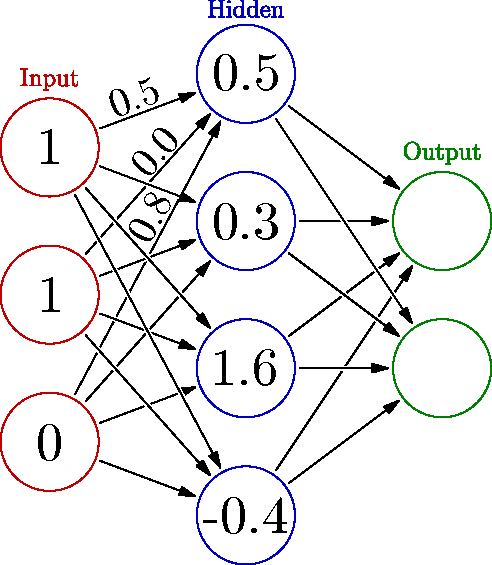
\includegraphics[height = \figheight]{./fig/3-layer_propagate_4.pdf}}
%   \caption{Glosser.ca / CC-BY-SA-3.0}
% \end{figure}
%     \end{block}
    \end{column}
  \end{columns}
\end{frame}



\begin{frame}
\frametitle{How does an artificial neural network run?}
\framesubtitle{By using maths, predictably!}
  \begin{columns}[T]
    \begin{column}{.45\textwidth}

     \begin{itemize}
\item \only<1>{But programmers are \emph{lazy}!} \only<2->{General names  save time}

%      \ \\   
     
     \ \\
     
%      \ \\
% \item We'd rather a computer did all the maths for us
%      \ \\
%      \ \\
%      \ \\
%           \ \\
     
     \item<3-> \textcolor{inputred}{input units:} $x_i$
          \ \\
     \ \\
     
     \item<4-> \textcolor{hiddenblue}{hidden units:} $a_j$
     \ \\
     \ \\
     
     \item<5-> \textcolor{outputgreen}{output units:} $y_k$
     \ \\
     \ \\
     \item<6-> connection weights:  $w_{ij}$ 
          \ \\
     \ \\
     \item<7-> subscripts \\ general: ${ijklm...}$ \\ specific: ${12345...}$

     \end{itemize}

% \only<7->{
%     \begin{overprint}
%         \onslide<7-9>
% 	\begin{equation*}
% 	a_i = \onslide<11->{f\left(} \onslide<9>{ \sum^{\textcolor{white}{N}}}   \onslide<8->{x_j \times w_{ji}}  \onslide<11->{\right)}
% 	\end{equation*}
% 	\onslide<10->
% 	\begin{equation*}
% 	a_i = \onslide<11->{f\left(}  \sum_{j=1}^N  x_j \times w_{ji}  \onslide<11->{\right)}
% 	\end{equation*}
%     \end{overprint}
% } 
    
% \only<12->{where $a_i$ is the unit whose state we want to calculate, $N$ is the number of units on the previous layer, $w_{ji}$ is the weight on the connection between $i$ and $j$, and $f$ is a function, commonly the logistic step function.}

% Which means, to calculate, e.g., $a_1$ multiply all the states in layer before with the incoming weight and then add them up. So in our case all the $x_1~...~x_3$ because $N = 3$.  
% \end{block}
    \end{column}
    \begin{column}{.55\textwidth}
%     \begin{block}{}
% Your image included here
	\begin{figure}[t]
	\begin{flushleft}
	
	\includegraphics<1-2>[height = \figheight]{./fig/3-layer.pdf}
% 	\includegraphics<>[height = \figheight]{./fig/3-layer.pdf}
% 	\includegraphics<3>[height = \figheight]{./fig/3-layer_maths_1.pdf}
	\includegraphics<3>[height = \figheight]{./fig/3-layer_maths_1.pdf}
	\includegraphics<4>[height = \figheight]{./fig/3-layer_maths_2.pdf}
	\includegraphics<5>[height = \figheight]{./fig/3-layer_maths_3.pdf}
	\includegraphics<6->[height = \figheight]{./fig/3-layer_maths.pdf}
% 	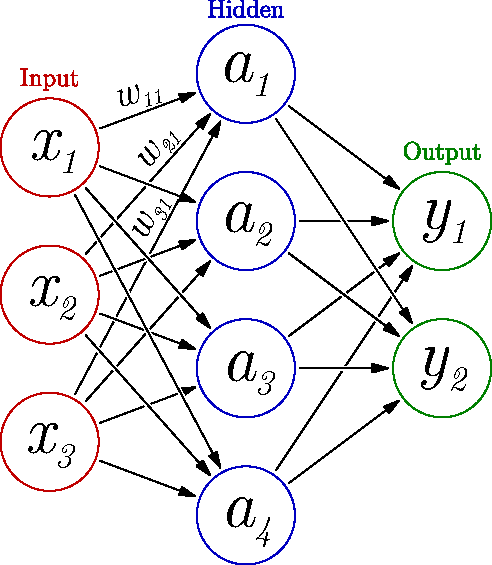
\includegraphics[height = \figheight]{./fig/3-layer_maths.pdf}
% 	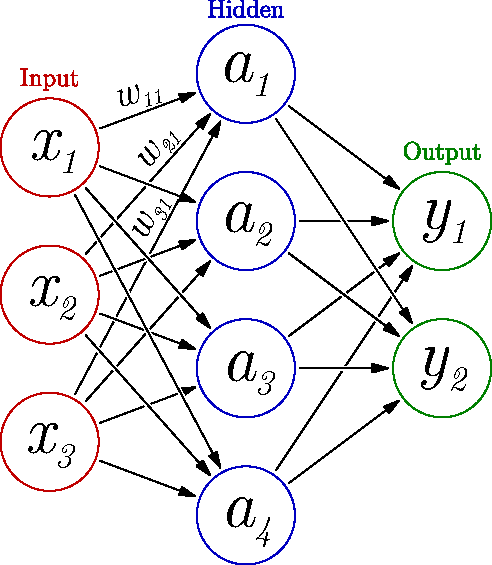
\includegraphics[height = \figheight]{./fig/3-layer_maths.pdf}
% 	  \caption{Glosser.ca / CC-BY-SA-3.0}
	\vspace{1cm}
	\end{flushleft}
	\end{figure}
%     \end{block}
    \end{column}
  \end{columns}
\end{frame}



\begin{frame}
\frametitle{How does an artificial neural network run?}
\framesubtitle{By using maths, predictably!}
  \begin{columns}[T]
    \begin{column}{.45\textwidth}
\ \\ 
\ \\ 
We use general names to write a general equation:

    \begin{overprint}
        \only<2>{
	\begin{equation*}
	a_i = \textcolor{white}{f\left(        \sum^N_{j=1} x_j \times w_{ji} \right)} 
	\end{equation*}}
         \only<3>{
	\begin{equation*}
	a_i = \textcolor{white}{f\left( \sum^N_{j=1} \textcolor{black}{ x_j \times w_{ji}  } \right)}
	\end{equation*}}
        \only<4>{
	\begin{equation*}
	a_i = \textcolor{white}{f\left( \textcolor{black}{ \sum^N_{j=1} x_j \times w_{ji}  } \right)}
	\end{equation*}}
	\only<5->{
	\begin{equation*}
	a_i = f\left(  \sum_{j=1}^N x_j \times w_{ji} \right)
	\end{equation*}}
    \end{overprint}
    
\only<6->{where $a_i$ is the unit whose state we want to calculate, $N$ is the number of units on the previous layer, $w_{ji}$ is the weight on the connection between $i$ and $j$, and $f$ is a function that the unit applies.}

% Which means, to calculate, e.g., $a_1$ multiply all the states in layer before with the incoming weight and then add them up. So in our case all the $x_1~...~x_3$ because $N = 3$.  
% \end{block}
    \end{column}
    \begin{column}{.55\textwidth}
%     \begin{block}{}
% Your image included here
	\begin{figure}[t]
	\begin{flushleft}
	
	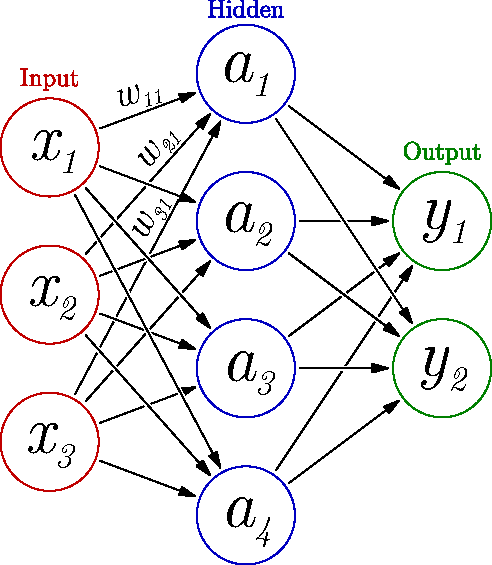
\includegraphics[height = \figheight]{./fig/3-layer_maths.pdf}
	\vspace{1cm}
	\end{flushleft}
	\end{figure}
%     \end{block}
    \end{column}
  \end{columns}
\end{frame}

\begin{frame}
\frametitle{How does an artificial neural network run?}
\framesubtitle{By using maths, predictably!}
  \begin{columns}[T]
    \begin{column}{.45\textwidth}
\ \\ 
\ \\ 
We use this equation by replacing \emph{iterators} $i$ and $j$:





	\begin{equation*}
	a_i = f\left(  \sum_{j=1}^N x_j \times w_{ji} \right)
	\end{equation*}
	
	
    \begin{overprint}
	\only<2>{
	\begin{equation*}
	a_{\textcolor{hiddenblue}{1}} = f\left(   \sum^N_{j=1} x_j \times w_{j\textcolor{hiddenblue}{1}} \right) 
	\end{equation*}
	}	
	\only<3-6>{
	\begin{equation*}
	a_{\textcolor{hiddenblue}{1}} = f\left(   \sum^{\textcolor{inputred}{3}}_{j=1} x_j \times w_{j\textcolor{hiddenblue}{1}} \right) 
	\end{equation*}
	
	}
	\only<7->{
	\begin{equation*}
	a_{\textcolor{hiddenblue}{2}} = f\left(   \sum^{\textcolor{inputred}{3}}_{j=1} x_j \times w_{j\textcolor{hiddenblue}{2}} \right) 
	\end{equation*}
	
	}
	

    \end{overprint}
\only<4-6>{
	\setlength{\tabcolsep}{1pt}
	\begin{tabular}{c c c}% syntax for siunitx v2; for v1 use "tabformat"
	\visible<4->{$x_{\textcolor{inputred}{1}} \times w_{\textcolor{inputred}{1}\textcolor{hiddenblue}{1}}$ }&\visible<5->{$+~ x_{\textcolor{inputred}{2}} \times w_{\textcolor{inputred}{2}\textcolor{hiddenblue}{1}}$}& \visible<6>{$+ ~ x_{\textcolor{inputred}{3}} \times w_{\textcolor{inputred}{3}\textcolor{hiddenblue}{1}}$}\\ 
	% \visible<17->{$-0.4 \times 1.1 ~=$ & $-0.44$ & + \\
	\end{tabular}
	}
	\only<8->{
	\setlength{\tabcolsep}{1pt}
	\begin{tabular}{c c c}% syntax for siunitx v2; for v1 use "tabformat"
	\visible<8->{$x_{\textcolor{inputred}{1}} \times w_{\textcolor{inputred}{1}\textcolor{hiddenblue}{2}}$ }&\visible<9->{$+~ x_{\textcolor{inputred}{2}} \times w_{\textcolor{inputred}{2}\textcolor{hiddenblue}{2}}$}& \visible<10>{$+ ~ x_{\textcolor{inputred}{3}} \times w_{\textcolor{inputred}{3}\textcolor{hiddenblue}{2}}$}\\ 
	% \visible<17->{$-0.4 \times 1.1 ~=$ & $-0.44$ & + \\
	\end{tabular}
	}
	
	
	
	
	

%      \begin{overprint}
%     	\only<4>{
% 	\begin{equation*}
% 	x_{\textcolor{inputred}{1}} \times w_{\textcolor{inputred}{1}\textcolor{hiddenblue}{1}} ~ \textcolor{purple}{ + x_{2} \times w_{21} + x_{3} \times w_{31}}
% 	\end{equation*}
% 	}	
%     	\only<5>{
% 	\begin{equation*}
% 	x_{\textcolor{inputred}{1}} \times w_{\textcolor{inputred}{1}\textcolor{hiddenblue}{1}} ~+ x_{\textcolor{inputred}{2}} \times w_{\textcolor{inputred}{2}\textcolor{hiddenblue}{1}} \textcolor{purple}{ + x_{3} \times w_{31}}
% 	\end{equation*}
% 	}
% 	\only<6>{
% 	\begin{equation*}
% 	x_{\textcolor{inputred}{1}} \times w_{\textcolor{inputred}{1}\textcolor{hiddenblue}{1}} ~ + x_{\textcolor{inputred}{2}} \times w_{\textcolor{inputred}{2}\textcolor{hiddenblue}{1}} + x_{\textcolor{inputred}{3}} \times w_{\textcolor{inputred}{3}\textcolor{hiddenblue}{1}}
% 	\end{equation*}
% 	}
%     \end{overprint}
    
% \only<7->{where $a_i$ is the unit whose state we want to calculate, $N$ is the number of units on the previous layer, $w_{ji}$ is the weight on the connection between $i$ and $j$, and $f$ is a function that the unit applies.}

% Which means, to calculate, e.g., $a_1$ multiply all the states in layer before with the incoming weight and then add them up. So in our case all the $x_1~...~x_3$ because $N = 3$.  
% \end{block}
    \end{column}
    \begin{column}{.55\textwidth}
%     \begin{block}{}
% Your image included here
	\begin{figure}[t]
	\begin{flushleft}
	
	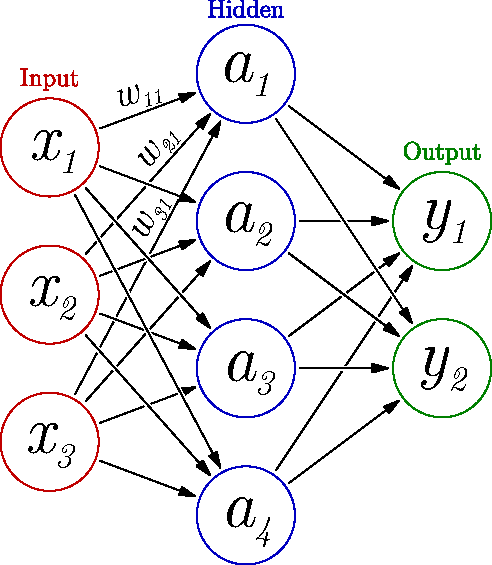
\includegraphics[height = \figheight]{./fig/3-layer_maths.pdf}
	\vspace{1cm}
	\end{flushleft}
	\end{figure}
%     \end{block}
    \end{column}
  \end{columns}
\end{frame}

\begin{frame}
\frametitle{How do networks learn?}
\framesubtitle{Cunning!}
\begin{itemize}
\item<1-> Many options: Hebbian learning, back-propagation of error, Boltzmann machine learning, self-organising map algorithm, etc. \\ \

\item<2-> All learning algorithms work by changing the connection weights \\ \

\item<3-> Learning can be divided into \emph{supervised}, \emph{unsupervised}, and \emph{reinforcement} \\ \ \end{itemize}
\end{frame}

\begin{frame}
\frametitle{Hebbian learning}
\framesubtitle{A very simple learning rule}
  \begin{columns}[T]
    \begin{column}{.45\textwidth}
    \ \\     \ \\     \ \\ 
%     \onslide<1->{
%     Units that are \emph{on} together in the pattern set are made to \emph{be} on together when the network is run:

     \onslide<1->{\small ``Cells that fire together, wire together'' \\ \
     --- Carla Shatz }
      \\ \
      \\ \
      \begin{center}
%       \begin{equation*}
	\uncover<5->{$\Delta$} \uncover<2->{$w_{i} =$} \uncover<4->{$\eta \times$} \uncover<3->{$\textcolor{inputred}{x_{i}} \times \textcolor{outputgreen}{y_j}$}
% 	\end{equation*}
     \end{center}



      
      
      \ \\      
      
      \ \\
      
      \onslide<6->{which means each weight is changed by a small in/decrement for every pattern}

%        \onslide<6-> {If $x_i$ or $a_j$ is on, then the other will also be on}
             

    \end{column}
    \begin{column}{.55\textwidth}
%     \begin{block}{}
% Your image included here
 \begin{figure}[t]
\centering
 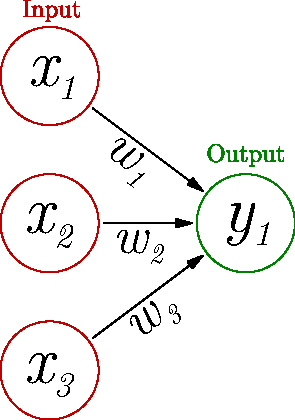
\includegraphics[height = \figheight]{./fig/perceptron_maths.pdf}
\end{figure}
    \end{column}
  \end{columns}
\end{frame}

\begin{frame}
\frametitle{Hebbian learning}
\framesubtitle{``Cells that fire together, wire together'' --- Carla Shatz }
  \begin{columns}[T]
    \begin{column}{.45\textwidth}
    \ \\ 
    \onslide<1->{{Hebb's rule is simple, but \emph{very unstable}!}}
      \ \\
      \mdseries
%     Units that are \emph{on} together in the pattern set are made to \emph{be} on together when the network is run:
	\only<2->{\begin{equation*}
	\Delta w_i = \eta  \times x_i  \times  y_j
	\end{equation*}}    
	\ \\	
	\ \\	
	\only<3->{\begin{center}
	$\Delta w_{1} = \only<9->{0.15} \only<3>{\eta} \only<4-8>{0.5} \only<3-8>{\times}  \only<3-4>{x_i} \only<5-6>{x_1} \only<7-8>{1.0}\only<3-8>{\times} \only<3-5>{y_j} \only<6-7>{y_1} \only<8>{0.3}$
	\end{center}}

%      \begin{overprint}
%         \only<3>{
% 	\begin{equation*}
% 	\Delta w_{1} = \eta \times  x_i  \times y_j
% 	\end{equation*}}
% 	\only<4>{
% 	\begin{equation*}
% 	\Delta w_{1} = 0.5 \times  x_i  \times y_j
% 	\end{equation*}}
% 	\only<5>{
% 	\begin{equation*}
% 	\Delta w_{1} = 0.5 \times  x_1  \times y_j
% 	\end{equation*}}
% 	\only<6>{
% 	\begin{equation*}
% 	\Delta w_{1} = 0.5 \times  x_1  \times y_1
% 	\end{equation*}}
% 	\only<7>{
% 	\begin{equation*}
% 	\Delta w_{1} = 0.5 \times  1.0  \times y_1
% 	\end{equation*}}
% 	\only<8>{
% 	\begin{equation*}
% 	\Delta w_{1} = 0.5 \times  1.0  \times 0.3
% 	\end{equation*}}
% 	\only<9-17>{
% 	\begin{equation*}
% 	\Delta w_{1} = 0.15
% 	\end{equation*}}
%     \end{overprint}
    
    \begin{center}
     

        \begin{overprint}
    	\only<10>{
%     	\begin{equation*}
	$\mathbf{new}~w_{1} = \mathbf{old}~ w_{1} + \Delta w_{1}$
% 	\end{equation*}
	}
    	\only<11>{
%     	\begin{equation*}
	$\mathbf{new}~w_{1} = 0.0 + \Delta w_{1}$
% 	\end{equation*}
	  }
    	\only<12>{
%     	\begin{equation*}
	$\mathbf{new}~w_{1} = 0.0 + 0.15$
% 	\end{equation*}}
	}
	\only<13>{
%     	\begin{equation*}
	$\mathbf{new}~w_{1} = 0.15$
% 	\end{equation*}
	  }
	  \only<14>{
%     	\begin{equation*}
	$w_{1} = 0.15$
% 	\end{equation*}
	  }
	  \only<15>{
%     	\begin{equation*}
	$w_{1} = 0.15$ + something positive
% 	\end{equation*}
	  }	\only<16>{
%     	\begin{equation*}
	$w_{1} = 0.15$ + something positive + something else positive +
% 	\end{equation*}
	  }	\only<17->{
%     	\begin{equation*}
	$w_{1} = 0.15$ + something positive + something else positive + another positive value + ...
% 	\end{equation*}
	  }
    \end{overprint}    
    \end{center}

% 	\begin{equation*}
% 	\Delta w_{11} = 0.5 \times  x_1  \times a_1
% 	\end{equation*}   
% 	
% 	\begin{equation*}
% 	\Delta w_{11} = 0.5 \times  1.0  \times a_1
% 	\end{equation*}  
% 	
% 	\begin{equation*}
% 	\Delta w_{11} = 0.5 \times  1.0  \times 0.3
% 	\end{equation*}  
% 	$\Delta w_{11} = x_1 \times  a_1 $
     
    \end{column}
    \begin{column}{.55\textwidth}
%     \begin{block}{}
% Your image included here
\begin{figure}[t]
 
\centering
 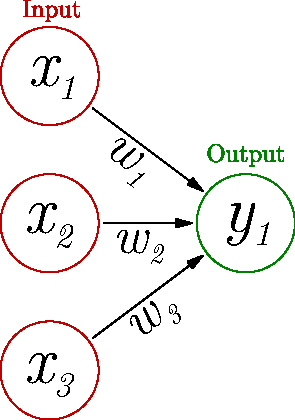
\includegraphics[height = \figheight]{./fig/perceptron_maths.pdf}
%   \caption{Glosser.ca / CC-BY-SA-3.0}
%     \end{block}

\end{figure}
%     \end{block}
    \end{column}
  \end{columns}
\end{frame}


\begin{frame}
\frametitle{The perceptron}
\framesubtitle{A simple classifier}
  \begin{columns}[T]
    \begin{column}{.45\textwidth}    \ \\ \ \\ 
    \ \\
    \begin{itemize}
    
 
     \item<2->Created in 1957 at the Cornell Aeronautical Laboratory by Frank Rosenblatt  \\ \
\item<3->Linear classifier \\ \

\item<4->Simplest form of feedforward network \\ \

% \item Consists of two layers of units \\ \
% \item No hidden units \\ \
\end{itemize}

    \end{column}
    \begin{column}{.55\textwidth}
\begin{figure}[t]
\centering
 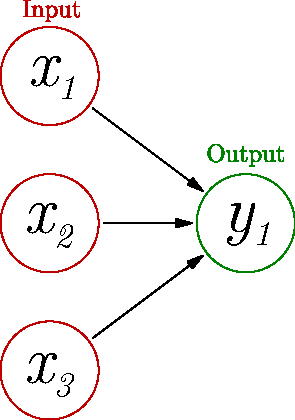
\includegraphics[height = \figheight]{./fig/perceptron.pdf}
\end{figure}
    \end{column}
  \end{columns}
\end{frame}


\begin{frame}
\frametitle{How does the perceptron learn?}
\framesubtitle{Maths again!}
  \begin{columns}[T]
    \begin{column}{.45\textwidth} 
    \ \\
    \ \\
\begin{enumerate}

 \item<1-> Initialise weights
 \\ \
 \item<2-> Run network \onslide<2>{using: 
 
 \begin{equation*}
y_j = f \left( \sum_1^N w_i \times x_i \right)
 \end{equation*} 
 \\ \
 
same as always!
\\ \
}

% \item<3-> Update weights using: 
%  
%  \begin{equation*}
%   \Delta w_i = \eta ( d_j - y_j ) \times x_{i}
%  \end{equation*} 
%   \ \\
%  
%  where $d$ is what we want $y$ to be given $x_i$, and $\eta$ is the learning rate.

 \end{enumerate}

    \end{column}
    \begin{column}{.55\textwidth}
%     \begin{block}{}
% Your image included here
\begin{figure}[t]
 \centering
 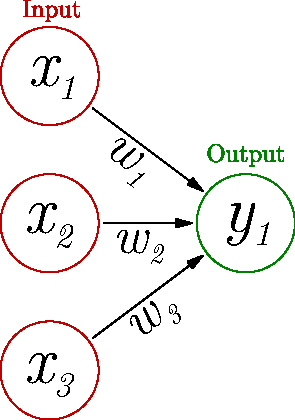
\includegraphics[height = \figheight]{./fig/perceptron_maths.pdf}
\end{figure}
    \end{column}
  \end{columns}
\end{frame}


\begin{frame}
\frametitle{How does the perceptron learn?}
\framesubtitle{Maths again!}
  \begin{columns}[T]
    \begin{column}{.45\textwidth} 
        \  \\
 \   \\ 
\begin{enumerate}
 \item Initialise weights
 
 \ \\
 \item Run network
 
 \ \\
 
 \item Update weights using:

\end{enumerate}
 
 \begin{center}
 $ \Delta w_i = \eta$ \only<2->{$( d_j - y_j )$} \only<1>{ $y_j $} $\times x_{i}$
 \end{center} 
  \ \\
 
 \only<3->{where $d$ is what we want $y$ to be given $x$, and $\eta$ is the learning rate.}

    \end{column}
    \begin{column}{.55\textwidth}
%     \begin{block}{}
% Your image included here
\begin{figure}[t]
\centering
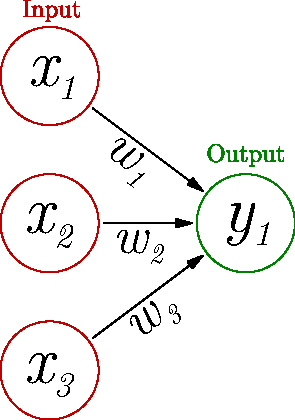
\includegraphics[height = \figheight]{./fig/perceptron_maths.pdf}
\end{figure}
%     \end{block}
    \end{column}
  \end{columns}
\end{frame}


\begin{frame}
\frametitle{How does the perceptron learn?}
\framesubtitle{Maths again!}
  \begin{columns}[T]
    \begin{column}{.45\textwidth} 
        \  \\
 \   \\ 
\begin{enumerate}
 \item<1-> Initialise weights
 
 \ \\
 \item<1-> Run network
 
 \ \\
 
 \item<1-> Update weights
 
  \ \\
 
 \item<1-> Repeat 2 and 3
 
 \ \\

 \item<2> When do we stop?
\end{enumerate}


    \end{column}
    \begin{column}{.55\textwidth}
%     \begin{block}{}
% Your image included here
\begin{figure}[t]
 \centering
 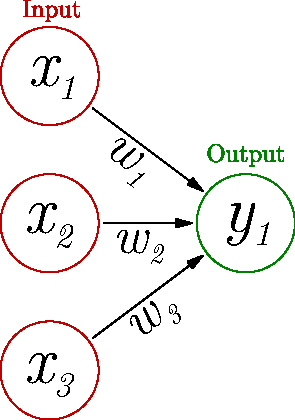
\includegraphics[height = \figheight]{./fig/perceptron_maths.pdf}
\end{figure}
    \end{column}
  \end{columns}
\end{frame}




\begin{frame}
\frametitle{Perceptron coding time}
\framesubtitle{}
        \  \\


 \Huge Time to program a perceptron!
 \   \\  \   \\ 
% \normalsize Oh, and join our mailing list so we can send you stuff: https://groups.google.com/d/forum/introcompcog

\end{frame}

\begin{frame}[fragile]
\frametitle{Training the network}
\framesubtitle{The basic algorithm!}
\begin{lstlisting}[style=base]
@1def Train(self):@          
@12   for t in range(100):@
@11       for p in range(P):@     
@3            for i in range(N):@
@2                x[i] = self.patterns[p][i]@
@6            y = 0@
@5            for i in range(N+1):@
@4                y += x[i] * w[i]@
@4            y = f(y)
@9            error = d[p][0] - y@
@10           for i in range(N+1):@
@9                w[i] += h * error * x[i]@
\end{lstlisting}

\end{frame}
\begin{frame}[fragile]
\frametitle{Training the network}
\framesubtitle{Defining some patterns!}
\begin{lstlisting}[style=base]
@Patterns =@
        @[#colour, shape, taste
         @@#red-yellow, big-small, sweet-sour
         @@[0.1, 0.0, 0.2], #loquat 
         @@[0.0, 0.2, 0.0], #lemon 
         @@[1.0, 0.5, 0.8], #red apple 
         @@[1.0, 0.0, 0.9], #strawberry 
        @@]@

@2Targets = [@
           @2[1.0], #first target
           @@2[1.0], #targets indicate 
           @@2[0.0], #which class
           @@2[0.0], #a pattern         
          @@2] #belongs to           
          @

\end{lstlisting}

\end{frame}
\end{document}
